% Copyright (C)  2018  TANSORIER.
% Permission is granted to copy, distribute and/or modify this document
% under the terms of the GNU Free Documentation License, Version 1.3
% or any later version published by the Free Software Foundation;
% with no Invariant Sections, no Front-Cover Texts, and no Back-Cover Texts.
% A copy of the license is included in the section entitled "GNU
% Free Documentation License".

% https://www.gnu.org/licenses/fdl-1.3.html

% compress option to have horyzontal circle
\documentclass[compress]{smilebeamer}

%%%%%%%%%%%%%%%%%%%%%%%%%%%%%%%%%%%%%%%%%%%%%%%%%%%%%%%%%%%%%%%%%%%%%

% Thèmes suppélmentaires
\useoutertheme[]{miniframes} % barre menu du haut
\setbeamertemplate{frametitle}[default] % replace le titre à la bonne place
\useinnertheme{rounded} % arrondi les angles

\setbeamertemplate{footline}[text line]{
\textcolor{gray}{%
	\parbox{\linewidth}{\vspace*{-8pt}Smile ECS\hfill\insertshortauthor\hfill\insertpagenumber/\inserttotalframenumber}}
}
\beamertemplatenavigationsymbolsempty

% Language
\usepackage[french]{babel}
\usepackage[utf8]{inputenc}
\usepackage[T1]{fontenc}

% Display Table Of Content spécific for smilebeamer
% Force to get empty
\AtBeginSection[]{}
\AtBeginSubsection[]{}
%{
%  \begin{frame}<beamer>
%  \frametitle{Plan}
%  \tableofcontents[currentsection]
%  \end{frame}
%}

% Change color of definiton block
\AtBeginEnvironment{definition}{%
	\setbeamercolor{block title}{use=example text,fg=example text.fg,bg=example text.fg!20!bg}
	\setbeamercolor{block body}{parent=normal text,use=block title,bg=block title.bg!50!bg}
}

% caption size reduce
\usepackage{caption}
\setbeamerfont{caption}{size=\scriptsize}

% code coloration
\usepackage{listings}
% L'option "[fragile]" doit être rajouté au frame pour pouvoir utiliser correctement
% la police verbatim
\usepackage{color}
\lstset{
  breaklines=true,
  tabsize=4,
  backgroundcolor=\color[RGB]{49,54,59},
  basicstyle=\footnotesize\ttfamily\color{white},
  commentstyle=\itshape\color[RGB]{0,136,136},
  morecomment=[l]{\#},
  morekeywords={*,\$,\{,\}},
  stringstyle=\itshape\color[RGB]{218,116,0},
  showstringspaces=false,
  frame=LTBR,
}
\lstdefinestyle{shell}{
  language=bash,
  keywords={\$},
  keywordstyle=\bfseries\color[RGB]{66,198,66},
  literate=
    {├}{{\smash{\raisebox{-1ex}{\rule{1pt}{\baselineskip}}}\raisebox{0.5ex}{\rule{1ex}{1pt}}}}1 
    {─}{{\raisebox{0.5ex}{\rule{1.5ex}{1pt}}}}1 
    {│}{{\smash{\raisebox{-1ex}{\rule{1pt}{\baselineskip}}}\raisebox{0.5ex}{\rule{1ex}{0pt}}}}1 
    {└}{{\smash{\raisebox{0.5ex}{\rule{1pt}{\dimexpr\baselineskip-1.5ex}}}\raisebox{0.5ex}{\rule{1ex}{1pt}}}}1
}
\lstdefinestyle{bitbake}{
  language=bash,
  alsoletter=-,
  morekeywords={\$,\{,\}},
  morekeywords={BBFILES,BBFILE_COLLECTIONS,BBFILE_PATTERN_meetup,BBFILE_PRIORITY_meetup,%
  BBLAYERS,MACHINE,DISTRO,LAYERDEPENDS_meta-python,DISTRO_FEATURES_remove,%
  DISTRO_FEATURES_append,VIRTUAL-RUNTIME_init_manager,require,DISTRO_NAME,%
  DISTRO_VERSION,DISTRO_FEATURES_DEFAULT,DISTRO_FEATURES_LIBC,PACKAGE_CLASSES,%
  POKY_DEFAULT_DISTRO_FEATURES,DISTRO_FEATURES,IMAGE_FEATURES,IMAGE_INSTALL},
  keywordstyle=\bfseries\color[RGB]{152,251,152},
}

% pour les schemas
\usepackage{tikz}
\usepackage{tikz}

% Pour utiliser des colonnes
\usepackage{multicol}

%%%%%%%%%%%%%%%%%%%%%%%%%%%%%%%%%%%%%%%%%%%%%%%%%%%%%%%%%%%%%%%%%%%%%
\title[Yocto]{Yocto - \texttt{devtool} - Ansible \\ \textbf{La dernière recette de ma grand-mère}}

\author[Mickaël Tansorier]{Mickaël Tansorier}

\date[Mars 2018]{Présenstation sur le fonctionnement de Yocto et d'outils pratiques.}
%%%%%%%%%%%%%%%%%%%%%%%%%%%%%%%%%%%%%%%%%%%%%%%%%%%%%%%%%%%%%%%%%%%%%

\begin{document}
%\tableofcontents[subsectionstyle=hide]

% *******************************
% ****     PAGE DE GARDE     ****
% *******************************

\begin{frame}
\titlepage
\end{frame}


% *******************************
% ****      INTRODUCTION     ****
% *******************************

\section{Introduction}

\begin{frame}
\underline{Objectif de la présentation}
\begin{itemize}
	\item Présenter Yocto
	\item Démonstration concrète sur Rapsberry Pi
	\item Présentation d'outils utiles
	\begin{itemize}
		\item \texttt{devtool}
		\item \texttt{Ansible}
	\end{itemize}
\end{itemize}
\end{frame}


\begin{frame}{Plan}
\tableofcontents[hideallsubsections]
\end{frame}


\subsection{Historique}

\begin{frame}{D'où vient ce nom ?}
\begin{definition}
	Yocto est un préfixe représentant 10\textsuperscript{-24} unités (SI)
\end{definition}
\end{frame}

\begin{frame}
\begin{block}{Qu'est ce qu'est vraiment Yocto ?}
	Yocto est un outil qui répond au besoin de générer une distribution
	\textbf{Linux embarqué} pour un matériel \textbf{dédié}.
\end{block}
\end{frame}

\begin{frame}
\begin{block}{Pourquoi Yocto existe ?}
	Ce projet s'est basé sur l'outil \textbf{OpenEmbedded} pour voir le jour.\newline{}\\
	En effet il y avait une volonté de pouvoir moduler les applications sur
	\textbf{différents matériels} sans avoir à investir dans un nouveau développement.
	\newline{}\\
	Des développeurs et la Fondation Linux se sont unis pour proposer	une 
	mécanique qui fasse abstraction du matériel, et ainsi rendre réutilisables
	les développements déjà effectués.\newline{}\\
	\textbf{Depuis 2010 ce projet continue sa route !}
\end{block}
\end{frame}


% *******************************
% ****     PRÉSENTATION      ****
% *******************************
\section{Présentation de Yocto}

\begin{frame}{Présentation de Yocto}
\begin{center}

\includegraphics[width=0.7\textwidth]{logos/yocto-project-transp.png}
\end{center}
\end{frame}

\begin{frame}{Pas si vite …}
Avant tout, un peut de contexte.\newline
\newline
\begin{itemize}
	\item Est-ce que Yocto est le seul outils qui existe ?
	\item Qu'est-ce qu'il a de plus que les autres ?
	\item ...
\end{itemize}
\end{frame}

%
% **** ALTERNATIVES ****
%
\subsection{Alternatives à Yocto}

\begin{frame}
D’autres outils permettent de créer des distributions Linux pour les systèmes embarqués.
\begin{columns}[t]
	\begin{column}{0.33\textwidth}
	\begin{exampleblock}{Buildroot}
		
\includegraphics[width=\textwidth]{logos/buildroot.png}
		Buildroot est un outil qui ressemble à un jeu de makefile, capable de générer tous les éléments pour démarrer un système sous Linux.
	\end{exampleblock} 
	\end{column}
	\begin{column}{0.33\textwidth}
	\begin{exampleblock}{Linux From Scratch}
		
\includegraphics[width=\textwidth]{logos/linux_from_scratch-with_text.png}
		\newline
		\newline
		Linux from scratch est un projet qui décrit pas à pas les instructions pour construire un système Linux. Très instructif mais fastidieux !
	\end{exampleblock}  
	\end{column}
	\begin{column}{0.33\textwidth}
	\begin{exampleblock}{OpenWrt}
		
\includegraphics[width=\textwidth]{logos/OpenWrt.png}
		\newline
		\newline
		\newline
		OpenWrt est un système libre et issu de Buildroot. Très orienté réseau, il offre la possibilité de gérer les paquets ipk.
	\end{exampleblock}   
	\end{column}
\end{columns} 
\end{frame}

%
% ****     LE PLUS DE YOCTO      ****
%
\subsection{Qu'est ce que Yocto a de plus ?}

\begin{frame}
	Yocto et Buildroot sont deux outils très proches mais avec fonctionnalité qui diffères en fonction des besoins
	\begin{center}
	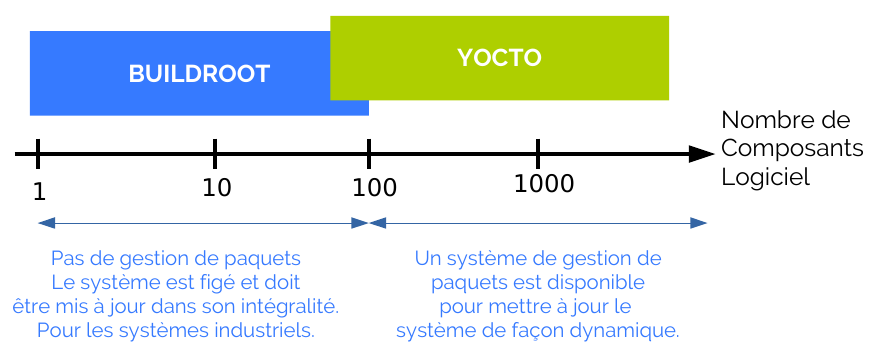
\includegraphics[width=0.7\textwidth]{schemas/buildroot_vs_yocto.png}	
	\end{center}
\end{frame}

\begin{frame}
La différenciation de l’\textbf{architecture matérielle} de l’\textbf{application logicielle} de la cible
\begin{itemize}
	\item \texttt{MACHINE} : définit l’architecture matérielle
	\item \texttt{DISTRO} : définit la distribution à générer
\end{itemize}
Une \textbf{communauté} active
\begin{itemize}
	\item Nouvelle version tous les 6 mois
	\item 1 version de dev, 3 stables, le reste en communauté
	\item Channel IRC actif
\end{itemize}
De la \textbf{documentation} bien fournie
\begin{itemize}
	\item Doc classique
	\item Vidéo
\end{itemize}
Des \textbf{outils} puissants
\begin{itemize}
	\item \texttt{devtool}
	\item \texttt{ipk}/\texttt{opkg}
\end{itemize}
\end{frame}

%
% ****     LE PLUS DE YOCTO      ****
%
\subsection{Configuration et Évolution}

\begin{frame}
\begin{itemize}
	\item Yocto est gourmand en ressources, une configuration minimale de 50Go de disque dur, un CPU à 1,6GHz et 8Go de RAM est recommandée.

	\item Plusieurs distributions Linux supportent Yocto : Ubuntu, Fedora, Debian, OpenSuse, CentOS.

	\item Le projet Yocto produit une nouvelle version majeure tous les 6 mois environ.

	\item Elle porte généralement un nom associé à un numéro de version.
ex : Morty (2.2), Pyro (2.3), Rocko (2.4), Sumo (2.5), ...
\end{itemize}
\end{frame}


\subsection{Le squelette}
\begin{frame}{Workflow}
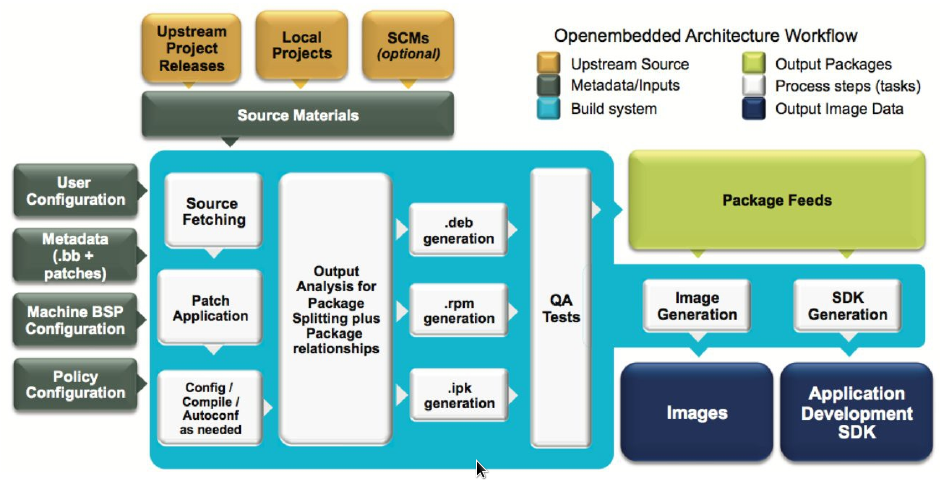
\includegraphics[width=\textwidth]{schemas/yocto_workflow.png}
\end{frame}

\begin{frame}
\tikzstyle{recette} = [draw, fill=smileOrange!70, rectangle, minimum height=2.5em, minimum width=10em,rounded corners=5pt]
\tikzstyle{cadre} = [rectangle, draw, minimum height=12em, minimum width=8.5em, fill=smileOrange!70]
\begin{center}
\begin{tikzpicture}[node distance=1.2cm]
% Yocto
\node[draw,rectangle,minimum height=8cm, minimum width=10cm, fill=smileOrange!70, label={[anchor=north]north:Yocto}] (YOCTO) {};
% Bitbake
\node[draw,rectangle, minimum height=2.5em, minimum width=8cm,rounded corners=5pt, fill=blue!40, yshift=2.8cm] (bitbake) {BITBAKE};
% Layers
\node[draw,rectangle, minimum height=2.5cm, minimum width=3cm,rounded corners=5pt, fill=green!70!black!70, yshift=0.7cm, xshift=-2cm, label={[anchor=north]north:LAYER A}] (layer-A) {};
\node[draw,rectangle, right of=layer-A, minimum height=2.5cm, minimum width=3cm,rounded corners=5pt, fill=green!70!black!70, xshift=2.6cm, label={[anchor=north]north:LAYER B}] (layer-B) {};
\node[draw,rectangle, below of=layer-A, minimum height=2.5cm, minimum width=3cm,rounded corners=5pt, fill=green!70!black!70, yshift=-1.8cm, label={[anchor=north]north:LAYER C}] (layer-C) {};
\node[draw,rectangle, below of=layer-B, minimum height=2.5cm, minimum width=3cm,rounded corners=5pt, fill=green!70!black!70, yshift=-1.8cm, label={[anchor=north]north:LAYER D}] (layer-D) {};
% Recettes
\node[draw,rectangle, below of=layer-A, fill=red!80!black!70, xshift=0.3cm, yshift=1.6cm] (rectte-A1) {RECETTE A1};
\node[draw,rectangle, below of=rectte-A1, fill=red!80!black!70, yshift=0.6cm] (rectte-A2) {RECETTE A2};
\node[draw,rectangle, below of=rectte-A2, fill=red!80!black!70, yshift=0.6cm] (rectte-A3) {RECETTE A3};
\node[draw,rectangle, below of=layer-B, fill=red!80!black!70, xshift=0.3cm, yshift=1.6cm] (rectte-B1) {RECETTE B1};
\node[draw,rectangle, below of=rectte-B1, fill=red!80!black!70, yshift=0.6cm] (rectte-B2) {RECETTE B2};
\node[draw,rectangle, below of=rectte-B2, fill=red!80!black!70, yshift=0.6cm] (rectte-B3) {RECETTE B3};
\node[draw,rectangle, below of=layer-C, fill=red!80!black!70, xshift=0.3cm, yshift=1.6cm] (rectte-C1) {RECETTE C1};
\node[draw,rectangle, below of=rectte-C1, fill=red!80!black!70, yshift=0.6cm] (rectte-C2) {RECETTE C2};
\node[draw,rectangle, below of=rectte-C2, fill=red!80!black!70, yshift=0.6cm] (rectte-C3) {RECETTE C3};
\node[draw,rectangle, below of=layer-D, fill=red!80!black!70, xshift=0.3cm, yshift=1.6cm] (rectte-D1) {RECETTE D1};
\node[draw,rectangle, below of=rectte-D1, fill=red!80!black!70, yshift=0.6cm] (rectte-D2) {RECETTE D2};
\node[draw,rectangle, below of=rectte-D2, fill=red!80!black!70, yshift=0.6cm] (rectte-D3) {RECETTE D3};
\end{tikzpicture}
\end{center}
\end{frame}

\begin{frame}
Quelques layers générique communautaire
\begin{itemize}
	\item meta
	\item meta-openembedded
	\begin{itemize}
		\item meta-oe
		\item meta-networking
		\item meta-python
		\item meta-gnome
	\end{itemize}
	\item meta-poky
\end{itemize}
D'autre plus spécifique
\begin{itemize}
	\item meta-raspberrypi
	\item meta-intel
	\item meta-xfce
	\item meta-qt5
\end{itemize}
\end{frame}


%
% ****     LE COEUR      ****
%
\subsection{Le coeur}

\begin{frame}
\begin{center}
\textcolor{smileOrange}{\huge{Avant de passer aux recettes, qui fait le travail dans Yocto ?}}
\end{center}
\end{frame}

\begin{frame}{bitbake}
\begin{block}{bitbake c'est quoi ?}
\begin{itemize}
	\item Un moteur d'exécution de tâches écrite en Python
	\item Fonctionne en ligne de commande
	\item Exécute automatiquement les tâches nécessaires à la fabrication de la cible fournie
\end{itemize}
\end{block}
\end{frame}


\begin{frame}{bitbake}
\tikzstyle{block} = [draw, fill=smileOrange!70, rectangle, minimum height=2.5em, minimum width=10em,rounded corners=5pt]
\tikzstyle{arrow} = [thick,->,>=stealth]
\begin{center}
\begin{tikzpicture}[node distance=1.2cm]
\node [block, fill=green!60!black!50]   (read)   {LECTURE RECETTE};
\node [block, below of=read]  (fetch)  {FETCH};
\node [block, below of=fetch] (unpack) {Unpack};
\node [block, below of=unpack] (patch) {PATCH};
\node [block, below of=patch] (configure) {CONFIGURE};
\node [block, right of=configure, xshift=3cm] (compile) {COMPILE};
\node [block, above of=compile] (install) {INSTALL};
\node [block, above of=install] (package) {PACKAGE};
\node [block, above of=package, fill=green!60!black!50] (rootfs) {ROOFS};

\draw[arrow] (read) -- (fetch);
\draw[arrow] (fetch) -- (unpack);
\draw[arrow] (unpack) -- (patch);
\draw[arrow] (patch) -- (configure);
\draw[arrow] (configure) -- (compile);
\draw[arrow] (compile) -- (install);
\draw[arrow] (install) -- (package);
\draw[arrow] (package) -- (rootfs);
\end{tikzpicture}
\end{center}
\end{frame}

\begin{frame}{recette}
\begin{block}{À quoi ça ressemble un recette ?}
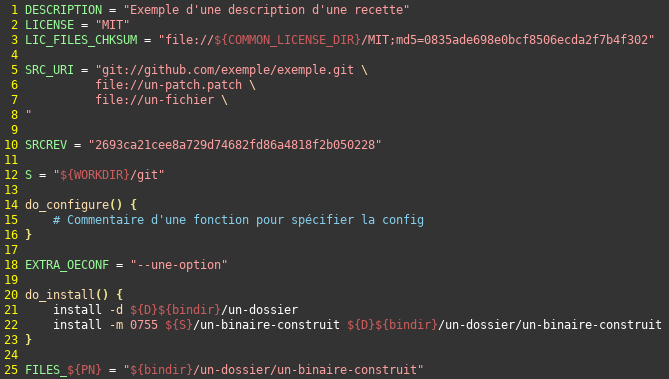
\includegraphics[width=\textwidth]{images/recette-yocto.png}
\end{block}
\end{frame}

%
% ****     CHOISIR UNE IMAGE      ****
%
\subsection{Se choisir une image}

\begin{frame}
\begin{center}
\textcolor{smileOrange}{\huge{Comment crée son image spécifique pour une carte donnée ?}}
\end{center}
\end{frame}

\begin{frame}
Yocto à la particularité de bien séparer la \textbf{distribution} de l'\textbf{architecture matériel}.
\newline \\
Les architectures matériel
\begin{itemize}
	\item ARM
	\item x86
	\item x86-64
	\item PowerPC
	\item MIPS
\end{itemize}
Les cartes associés
\begin{itemize}
	\item Raspberry Pi (différent versions)
	\item Beaglebone
	\item intel-core2-32
\end{itemize}
\textcolor{gray}{\tiny{Les différents BSP sont répertoriés sur le site de yoctoproject : https://www.yoctoproject.org/downloads/bsps}}
\end{frame}

\begin{frame}[fragile]
Le paramétrage de la \texttt{DISTRO} et de la \textsl{MACHINE} se fait en local.
\newline \\
\texttt{\$POKY/build/conf/local.conf}
\begin{lstlisting}[style=bitbake]
# This sets the default machine to be qemux86 if no other machine is selected:
MACHINE ??= "qemux86"
# Default distro:
DISTRO ?= "poky"

# Mes parametres
MACHINE = "raspberrypi3"
DISTRO = "distromeetup"
\end{lstlisting}
\end{frame}


% *******************************
% ****    TP RASPBERRY PI    ****
% *******************************
\section{TP Rapsberry Pi}

\begin{frame}{TP Raspberry Pi}
\begin{center}

\includegraphics[width=0.9\textwidth]{logos/yocto_plus_raspberry_pi.png}
\end{center}
\end{frame}

\subsection{installer l'invironnement yocto}
\begin{frame}{TP Raspberry Pi}
\begin{itemize}
	\item installer l'environnement
	\item construire une distribution générique
	\item créer sa propre distribution
	\item tester son image
\end{itemize}
\end{frame}

\subsection{installer l'environnement yocto}
\begin{frame}[fragile]
On se base sur la dernière version de yocto stable disponible, c'est à dire rocko qui est sortie en octobre 2017. (la prochaine est en avril 2018)
\begin{lstlisting}[style=shell]
$ git clone git://git.yoctoproject.org/poky -b rocko
$ cd poky
$ git clone git://git.yoctoproject.org/meta-raspberrypi -b rocko
$ git clone git://git.openembedded.org/meta-openembedded -b rocko
\end{lstlisting}
\end{frame}

\subsection{construire une distribution générique}
\begin{frame}[fragile]
Il faut maintenant paramétré la \texttt{MACHINE} et la \texttt{DISTRO} que l'on souhaite.\newline
Il faut tout d'abord sourcer son environnement afin que bitbake ait connaissance des variable de paramétrage.\newline
Ces variables sont écrites dans le fichier \texttt{local.conf} et \texttt{bblayers.conf}.\newline
\newline
Pour les générer il faut utiliser le scripte de yocto:
\begin{lstlisting}[style=shell]
$ . oe-init-build-env
\end{lstlisting}
Cela nous créer un dossier \texttt{build} dans lequel tout va se passer.
\end{frame}

\begin{frame}[fragile]
	Il reste plus qu'à modifier \texttt{\$POKY/build/conf/local.conf}
\begin{lstlisting}[style=bitbake]
# Mes parametres
MACHINE = "raspberrypi3-64"
\end{lstlisting}
et \texttt{\$POKY/build/conf/bblayers.conf}
\begin{lstlisting}[style=bitbake]
BBLAYERS += " \
    ${TOPDIR}/../meta-raspberrypi \
    ${TOPDIR}/../meta-openembedded/meta-python \
    ${TOPDIR}/../meta-openembedded/meta-oe \
"
\end{lstlisting}
\textcolor{gray}{\tiny{Les chemains sont en général absolue comme: \texttt{/home/username/path/to/project/poky/meta-raspberrypi}}}\newline
Et enfin lancer la construction de l'image avec
\begin{lstlisting}[style=shell]
$ bitbake core-image-minimal
\end{lstlisting}
\end{frame}


\subsection{Yocto est intelligent}
\begin{frame}[fragile]
Yocto est là pour vous aider à construire votre image.\newline
En effet si l'on ne rajoute seulement \texttt{meta-raspberrypi} dans \texttt{bblayers.conf} on obtiens l'erreur suivante:

\begin{block}{meta-python}
\begin{lstlisting}[basicstyle=\footnotesize\ttfamily\color{red!80!black!60}]
ERROR: ParseError at /home/ubuntu/meetup/poky/meta-raspberrypi/recipes-devtools/python/rpio_0.10.0.bb:9: Could not inherit file classes/pypi.bbclass
\end{lstlisting}
Il faut donc rajouter \texttt{meta-openembedded/meta-python}
\end{block}

\begin{block}{meta-oe}
\begin{lstlisting}[basicstyle=\footnotesize\ttfamily\color{red!80!black!60}]
ERROR: Layer 'meta-python' depends on layer 'openembedded-layer', but this layer is not enabled in your configuration
\end{lstlisting}
De plus dans \texttt{meta-python/conf/layer.conf} on a
\begin{lstlisting}[style=bitbake]
LAYERDEPENDS_meta-python = "core openembedded-layer"
\end{lstlisting}
\end{block}
\end{frame}


\subsection{Créer sa propre distribution}
%https://www.yoctoproject.org/docs/2.5/mega-manual/mega-manual.html#enabling-wayland-in-an-image
\begin{frame}
\begin{center}
\textcolor{smileOrange}{\huge{Créer sa propre distribution}}
\end{center}
\end{frame}

\begin{frame}[fragile]
Pour créer sa propre distribution il est préférable de créer son propre layer
\begin{lstlisting}[style=shell]
$ cd $POKY
$ mkdir -p meta-meetup/conf
\end{lstlisting}

Il faut déclarer la layer avec \texttt{./conf/layer.conf}
\begin{lstlisting}[style=bitbake]
# We have a conf and classes directory, add to BBPATH
BBPATH .= ":${LAYERDIR}"

# We have recipes-* directories, add to BBFILES
BBFILES += "${LAYERDIR}/recipes-*/*/*.bb \
            ${LAYERDIR}/recipes-*/*/*.bbappend"

BBFILE_COLLECTIONS += "meetup"
BBFILE_PATTERN_meetup = "^${LAYERDIR}/"
BBFILE_PRIORITY_meetup = "10"
\end{lstlisting}
\end{frame}

\begin{frame}[fragile]
Il faut maintenant l'ajouter dans \texttt{\$POKY/build/conf/bblayers.conf}
\begin{lstlisting}[style=bitbake,escapeinside={<@}{@>}]
BBLAYERS += " \
    ${TOPDIR}/../meta-raspberrypi \
    ${TOPDIR}/../meta-openembedded/meta-python \
    ${TOPDIR}/../meta-openembedded/meta-oe \
    <@\textit{\texttt{\textcolor{red}{\$\{TOPDIR\}/../meta-meetup}}}@> \
"
\end{lstlisting}
\end{frame}

\begin{frame}[fragile]
Créer sa distro avec \texttt{./conf/distro/distromeetup.conf}
\begin{lstlisting}[style=bitbake]
# Distribution base sur poky
require conf/distro/poky.conf

DISTRO = "distromeetup"
DISTRO_NAME = "Distro example"
DISTRO_VERSION = "0.1"

# Ajout d'option pour la distribution
DISTRO_FEATURES_append = " systemd"
VIRTUAL-RUNTIME_init_manager = "systemd"

# Utilisation seulement du paquetage ipk
PACKAGE_CLASSES = "package_ipk"
\end{lstlisting}

Si on souhaite utiliser la nouvelle distribution il faut ajouter dans \texttt{\$POKY/build/conf/local.conf}
\begin{lstlisting}[style=bitbake]
MACHINE = "raspberrypi3_64"
DISTRO = "distromeetup"
\end{lstlisting}
\end{frame}

\begin{frame}
\begin{center}
\textcolor{smileOrange}{\huge{Créer son image et choisir ce que l'on met dedans ?}}
\end{center}
\end{frame}

\begin{frame}[fragile]
	Par defaut la distro héritant de poky contiens
	\begin{lstlisting}[style=bitbake]
DISTRO_FEATURES = "${DISTRO_FEATURES_DEFAULT} ${DISTRO_FEATURES_LIBC} ${POKY_DEFAULT_DISTRO_FEATURES}"
	\end{lstlisting}
	
\end{frame}

\begin{frame}[fragile]
	Avec dans chaques variables
	\begin{lstlisting}[style=bitbake]
DISTRO_FEATURES_DEFAULT="acl alsa argp bluetooth ext2 irda largefile pcmcia usbgadget us      bhost wifi xattr nfs zeroconf pci 3g nfc x11"
	
DISTRO_FEATURES_LIBC="ipv4 ipv6 libc-backtrace libc-big-macros libc-bsd libc-cxx-tests l      ibc-catgets libc-charsets libc-crypt libc-crypt-ufc libc-db-aliases libc-envz libc-fcvt libc-fmtmsg libc-fstab libc-ftraverse libc-getlogin libc-idn libc-inet-anl libc-libm libc-locales libc-locale-code libc-memusage libc-nis libc-nsswitch libc-rcmd libc-rtld-debug libc-spawn libc-streams libc-sunrpc libc-utmp libc-utmpx libc-wordexp libc-posix-clang-wchar libc-posix-regexp libc-posix-regexp-glibc libc-posix-wchar-io"
	
POKY_DEFAULT_DISTRO_FEATURES="largefile opengl ptest multiarch wayland vulkan"
	\end{lstlisting}
\end{frame}

\begin{frame}[fragile]
Créer son image \texttt{./recipes-image/rapsberrypi/myrpi.bb}
\begin{lstlisting}[style=bitbake]
require recipes-graphics/images/core-image-weston.bb
IMAGE_FEATURES += " 
    ssh-server-openssh \
"
IMAGE_INSTALL += " \
    setkey \
"
\end{lstlisting}
{\color[RGB]{232,120,0}\texttt{ssh-server-openssh}} permet d'avoir accès à la carte en ssh
{\color[RGB]{232,120,0}\texttt{setkey}} nouvelle recette permettant de passer qwerty en bépo
\end{frame}



% *******************************
% ****    OUTILS DEVTOOL    ****
% *******************************
\section{Outils \texttt{devtool}}

\begin{frame}{\texttt{devtool}}
\tableofcontents[currentsection,hideallsubsections]
\end{frame}

\begin{frame}{\texttt{devtool}}
\begin{center}
\textcolor{smileOrange}{\huge{Exemple de l'utilisation de l'outil \texttt{devtool}}}
\end{center}
\end{frame}

\subsection{Les commandes de bases}

\begin{frame}
\texttt{devtool} est un outils très utiles lorsque l'on souhaite créer, développer ou modifier un recette et ses sources.\newline
Les commandes de base:
\begin{description}
	\item[\texttt{devtool add}] Ajoute un nouveau software à construir
	\item[\texttt{devtool modify}] Génère un environnement pour modifier les sources d'une composant
	\item[\texttt{devtool upgrade}] Met à jour une recette existante
\end{description}
\end{frame}

\begin{frame}
Les sources peuvent provenir de plusieurs endroits différent
\begin{center}
	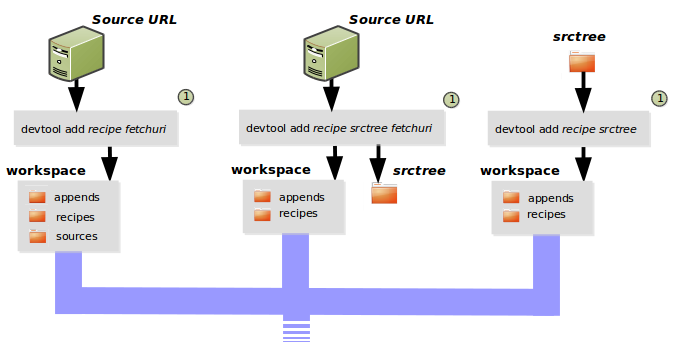
\includegraphics[width=1\textwidth]{images/devtool-add-src.png}
\end{center}
\end{frame}

\begin{frame}
De même pour modifier une recette
\begin{center}
	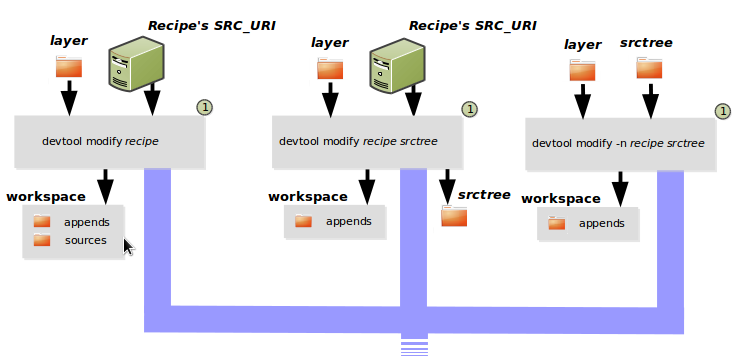
\includegraphics[width=1\textwidth]{images/devtool-modify-src.png}
\end{center}
\end{frame}

\subsection{Le comportement de \texttt{devtool}}

\begin{frame}[fragile]
Dès lors devtool créer une layers spéciale (\texttt{workspace}) qui prend la priorité maximal sur les autres layers
\begin{lstlisting}[style=shell,breaklines=false,xleftmargin=-18px,xrightmargin=-18px]
$ bitbake-layers show-layers
NOTE: Starting bitbake server...
layer              path                                      priority
=========================================================================
meta               /home/[...]/meta                          5
meta-poky          /home/[...]/meta-poky                     5
meta-yocto-bsp     /home/[...]/meta-yocto-bsp                5
workspace          /home/[...]/build/workspace               99
meta-raspberrypi   /home/[...]/build/../meta-raspberrypi     9
meta-python        /home/[...]/build/../meta-openembedded/meta-python  7
meta-oe            /home/[...]/build/../meta-openembedded/meta-oe  6
meta-meetup        /home/[...]/build/../meta-meetup           10
\end{lstlisting}
\end{frame}

\begin{frame}[fragile]
Dans ce layer on retrouve
\begin{itemize}
	\item les sources mis sous git et patché
	\item un bbappend de la recette
\end{itemize}
\begin{lstlisting}[style=shell]
$ cd $POKY/build/workspace/
$ tree -L 2 
.
├── appends
│   └── weston_2.0.0.bbappend
├── conf
│   └── layer.conf
├── README
└── sources
    └── weston
\end{lstlisting}
\end{frame}

\subsection{Exemple pratique}

\begin{frame}
\begin{center}
\textcolor{smileOrange}{\huge{Exemple pratique avec la recette \texttt{weston}}}
\end{center}
\end{frame}

\begin{frame}[fragile]
Modification avec \texttt{devtool} des sources de weston
\begin{lstlisting}[style=shell]
$ devtool modify weston
$ cd $POKY/build/workspace/sources/weston/
$ vim libweston/compositor-wayland.c +1655
\end{lstlisting}

Ajout du patch "Fix an uninitialized variable"
% https://github.com/wayland-project/weston/commit/6b2fb180d99bb9d6deaddb1cdf735422d4dd5b93
\begin{lstlisting}[escapeinside={<@}{@>}]
@@ -1652,6 +1652,7 @@ input_handle_axis(void *data, struct wl_pointer *pointer,
 
 	weston_event.axis = axis;
 	weston_event.value = wl_fixed_to_double(value);
<@\textcolor{green!80!black}{\texttt{+\,\,\,\, weston\_event.has\_discrete = false;}}@>
 
 	if (axis == WL_POINTER_AXIS_VERTICAL_SCROLL &&
 	    input->vert.has_discrete) {
\end{lstlisting}
\end{frame}

\begin{frame}[fragile]
Les étapes
\begin{enumerate}
\item Faire la modification
\item Tester
\item Appliquer la modification sous forme de patch
\begin{lstlisting}[style=shell]
$ devtool update-recipe weston
[...]
NOTE: Adding new patch 0001-Fix-an-uninitialized-variable.patch
NOTE: Updating recipe weston_2.0.0.bb
\end{lstlisting}
\item Ajouter la modification dans son layer
	% L'ajout d'un bbappend dans meta-meetup
	% Supprimer l'ajout de meta/recipes-graphics/wayland/weston_2.0.0.bb
	% Le déplacement du patch dans meta-meetup
\item Arrêter devtool
\begin{lstlisting}[style=shell]
$ devtool reset weston
\end{lstlisting}
\end{enumerate}
\end{frame}



% *******************************
% ****     OUTILS ANSIBLE    ****
% *******************************
\section{Outils Ansible}

\begin{frame}{Ansible}
\tableofcontents[currentsection,hideallsubsections]
\end{frame}

\begin{frame}
\begin{center}
\textcolor{smileOrange}{\huge{Utiliser Ansible pour mettre en place un environnement Yocto}}
\end{center}
\end{frame}

\subsection{C'est quoi Ansible ?}

\begin{frame}
\begin{definition}
Ansible est un logiciel destiné à la configuration et la gestion de parc informatique.
\end{definition}
Il permet de :
\begin{itemize}
	\item déployer des logiciels
	\item gérer des configurations
	\item lancer des tâches
\end{itemize}
\begin{itemize}
	\item[] Sur
	\begin{itemize}
	\item une machine
	\item plusieurs machines
	\end{itemize}
\end{itemize}
\end{frame}

\begin{frame}
	Un des avantage est qu'il utilise des fichiers de configuration au format YAML.
\begin{itemize}
	\item YAML est humainement lisibles
	\item et plus facile à géré que certain autres formats
\end{itemize}
\end{frame}

\subsection{Exemple simple de syntaxe}

\begin{frame}[fragile]
Défénition des cibles dans \texttt{/etc/ansible/hosts}
\begin{lstlisting}
192.0.2.50
linuxembedded.exemple.fr
\end{lstlisting}
\end{frame}

\begin{frame}[fragile]
Pour lancer un programme à distance on peux soit spécifier
\begin{itemize}
	\item tout les hôtes
	\item un hôte particulier
\end{itemize}
\begin{lstlisting}[style=shell]
$ ansible all -a "/bin/ping 8.8.8.8 -c1"
$ ansible linuxembedded.exemple.fr -a "/bin/ping 8.8.8.8 -c1"
\end{lstlisting}
\end{frame}

\begin{frame}[fragile]
Ansible fournit un ensemble de modules\newline
Qui permettent de lancer de action spécifique à distance
\begin{lstlisting}[style=shell]
$ ansible all -m ping
<address_ip> | SUCCESS => {
 "changed": false, 
 "ping": "pong"
}
\end{lstlisting}
\textcolor{gray}{\tiny{Attention au faux amis, ici ping se connecte à un hôte, teste l’utilisabilité de python puis de renvoie le résultat pong en cas de succès}}
\end{frame}

\subsection{Le playbook}

\begin{frame}
\begin{center}
\textcolor{smileOrange}{\huge{Les actions multiples – le principe de playbook}}
\end{center}
\end{frame}

\begin{frame}[fragile]
Pour effectuer plusieurs actions en une seule commande on utilise un playbook
\begin{lstlisting}[style=shell]
$ ansible-playbook mon-fichier.yml
\end{lstlisting}
\end{frame}

\begin{frame}
\begin{center}
\textcolor{smileOrange}{\huge{La syntaxe YAML}}
\end{center}
\end{frame}

\begin{frame}
\begin{exampleblock}{Buildroot}
Le standard YAML a été créé en 2001 et est utilisé dans divers projets.
\end{exampleblock}
Un fichier YAML est formé de
\begin{itemize}
	\item variables
	\item dictionnaires (clé/valeur)
	\item listes
\end{itemize}
\end{frame}

\begin{frame}[fragile]{Les variables}
Déclaration
\begin{lstlisting}[style=shell]
vars:
  base_path: /mon/path
\end{lstlisting}
Accès à la varible
\begin{lstlisting}[style=shell]
{{ base_path }}
\end{lstlisting}
Il est conseillé d'entourer la varible de guillemets
\begin{lstlisting}[style=shell]
app_path: "{{ base_path }}/app"
\end{lstlisting}
Passer les variables en ligne de commande avec l'option
\begin{lstlisting}[style=shell]
--extra-vars "base_path=/mon/path/"
\end{lstlisting}
\end{frame}

\begin{frame}[fragile]{Les dictionnaires}
Les dictionnaires sont définis sous la forme \textit{\texttt{clé: valeur}}.
\begin{lstlisting}[style=bitbake]
# Information sur une personne
 martin:
   nom: Martin Devloper
   travail: Developer
   niveau: Experimente
\end{lstlisting}
\end{frame}

\begin{frame}[fragile]{Les listes}
Les listes sont définies avec \textit{\texttt{-␣}}, un tiret suivi d’un espace.
\begin{lstlisting}[style=bitbake]
# Une liste de fruits
 - Pomme
 - Orange
 - Framboise
 - Mangue
\end{lstlisting}
\end{frame}

\begin{frame}[fragile]{Mélangeant des différentes syntaxes}
D’autres choses plus complexes sont possibles en mélangeant les différentes syntaxes:
\begin{lstlisting}[style=bitbake]
# Liste de plusieurs employes
- martin:
  nom: Martin D'vloper
  travail: Developer
  competences:
    - python
    - perl

- tabitha:
  nom: Tabitha Bitumen
  travail: Developer
  competences:
    - lisp
    - fortran
\end{lstlisting}
\end{frame}


\begin{frame}[fragile]{Les modules}
Les modules lut par Ansible sont déclaré sous la forme \textit{\texttt{clé: valeur}}.\newline
Voici une liste non exhaustive de types de modules disponibles :
\begin{multicols}{2}
\begin{itemize}
	\item git
	\item patch
	\item get\_url
	\item shell
	\item copy
	\item service
	\item apt
	\item yum
	\item lxc\_container
	\item make
\end{itemize}
\end{multicols}
\end{frame}


\begin{frame}[fragile]{Exemple}
Le module \texttt{git} utilise de sous-options
\begin{lstlisting}[style=bitbake]
# Exemple d'un telechargement de source git
- git:
  repo: 'https://git.yoctoproject.org/git/poky'
  version: krogoth
  dest: /home/user/poky
\end{lstlisting}
D'autres sous-options:
\begin{itemize}
	\item \texttt{update: yes}
	\item \texttt{archive: /path/to/archive.zip}
	\item ...
\end{itemize}
\end{frame}

\begin{frame}[fragile]{Module particulier: hosts}
Ce module est obligatoire.\newline
il fait référence aux hôtes dans \texttt{/etc/ansible/hosts}.
\begin{lstlisting}[style=bitbake]
- hosts: all
  remote_user: root
\end{lstlisting}
\end{frame}

\subsection{Ansible avec Yocto}

\begin{frame}
\begin{center}
\textcolor{smileOrange}{\huge{Comment utilisé Ansible pour déployer un environnement de développement pour Yocto ?}}
\end{center}
\end{frame}

\begin{frame}[fragile]{Définir l'hôte}
On utilise le \texttt{hosts} local
\begin{lstlisting}[style=bitbake]
- hosts: 127.0.0.1
  connection: local
\end{lstlisting}
\end{frame}

\begin{frame}[fragile]{Répertoire de travail}
Pour centraliser les sources on utilise un variable \texttt{TOP\_SRCDIR}.\newline
Elle sera passé en paramètre de la commande Ansible
\begin{lstlisting}[style=shell]
--extra-vars "TOP_SRCDIR=<path_to_top_srcdir>"
\end{lstlisting}
Ce qui donnera
\begin{lstlisting}[style=bitbake]
- name: "Get poky"
  git:
    repo: https://git.yoctoproject.org/git/poky
    version: krogoth
    dest: "{{TOP_SRCDIR}}"
\end{lstlisting}
\end{frame}

\subsection{Exemple complet}
\begin{frame}[fragile]
\begin{lstlisting}[style=bitbake,basicstyle=\tiny\ttfamily\color{white}]
- name: "Mon Projet"
  hosts: 127.0.0.1
  connection: local
  tasks:

  - name: "Get poky"
    git:
      repo: https://git.yoctoproject.org/git/poky
      version: krogoth
      dest: "{{TOP_SRCDIR}}"
      update: no

  - name: "Patch poky krogoth"
    patch:
      src: ../0001-qemu-Add-space-to-fix-concatenated-SRC_URI.patch
      basedir: "{{TOP_SRCDIR}}"
      strip: 1

  - name: "Copy hooks into poky"
    copy:
      src: /path/to/hooks/commit-msg
      dest: "{{TOP_SRCDIR}}/.git/hooks/commit-msg"
      mode: 755

  - name: "Get toolchain"
    get_url:
      url: http://192.168.2.200/src/toolchain/toolchain-M2.1.tgz
      checksum: md5:31a70bd7f7b74724af915a88fbe64f3d
      dest: "{{TOP_SRCDIR}}"

  - name: "Untar toolchain"
    shell: tar xzf {{TOP_SRCDIR}}/toolchain-M2.1.tgz -C {{TOP_SRCDIR}}/sdk/prebuilts/gcc/
\end{lstlisting}
\end{frame}

\begin{frame}[fragile]{Lancer}
Pour lancer le projet
\begin{lstlisting}[style=shell]
$ ansible-playbook mon-fichier.yml --extra-vars "TOP_SRCDIR=/home/user/mon-projet/"
\end{lstlisting}

\begin{lstlisting}[style=shell,basicstyle=\tiny\ttfamily\color{white}]
$ tree poky
poky/
.
├──  bitbake
├──  build
├──  documentation
├──  LICENSE
├──  meta
├──  meta-poky
├──  meta-selftest
├──  meta-skeleton
├──  meta-yocto
├──  meta-yocto-bsp
├──  oe-init-build-env
├──  oe-init-build-env-memres
├──  README
├──  README.hardware
├──  sdk
├──  scripts
└──  toolchain-M2.1.tgz
\end{lstlisting}
\end{frame}



% *******************************
% ****     CONCLUSION    ****
% *******************************

\begin{frame}
\begin{center}
\huge{Merci de votre attention !}
\end{center}
\begin{center}
Quetions ?
\end{center}
\end{frame}

\end{document}
